\documentclass[11pt,a4paper]{article}
\usepackage[utf8]{inputenc}
\usepackage[T1]{fontenc}
\usepackage{polski}
\usepackage{lmodern}
\usepackage[a4paper,margin=2cm]{geometry}
\usepackage{amsmath,amssymb}
\usepackage{graphicx}
\usepackage{booktabs,array}
\usepackage{caption}
\usepackage{microtype}
\usepackage{xcolor}
\usepackage{enumitem}
\usepackage{etoolbox}
\usepackage[colorlinks=true,linkcolor=blue,urlcolor=blue]{hyperref}
\graphicspath{{./}{../}{../../knowles_reframe/figures/}}
\emergencystretch=3em
\captionsetup{font=small,labelfont=bf}
\setlength{\parskip}{4pt}
\setlength{\parindent}{0pt}
\setlist{itemsep=2pt,topsep=3pt}
\newcommand{\citone}[1]{\citsep\ref{#1}\gdef\citsep{,\,}}
\newcommand{\cit}[1]{[\gdef\citsep{}\forcsvlist{\citone}{#1}]}
\newcommand{\ramka}[1]{\par\smallskip\noindent\fcolorbox{gray!60}{gray!7}{\parbox{\dimexpr\linewidth-2\fboxsep-2\fboxrule}{#1}}\par\smallskip}

\title{Sód, PEG i hybrydyzacja DNA\\\large co mówi NMR, co zakłada nasz model, jak to robi Knowles\\i jak to rozstrzygnąć eksperymentem}
\author{Wersja „prostym językiem”\\\small szczegóły i źródła: \texttt{report.pdf}, \texttt{na\_notes.md}, \texttt{mg\_notes.md}}
\date{11 października 2026}

\begin{document}
\maketitle
\vspace{-1.5em}

\ramka{\textbf{W sześciu zdaniach.}
(1) NMR pokazuje, że EG i PEG 200 \emph{nie} wiążą sodu, a długie PEG wiążą go słabo; nie mówi jednak, jak bardzo to zmienia ekranowanie DNA.
(2) Nasz model zamienia spowolnienie sodu z NMR wprost na „mniej sodu dla DNA”, ale pomija anion i liczy to w sposób, który przeszacowuje efekt około 3 razy.
(3) Pomiary termodynamiczne z literatury (VPO) pokazują, że PEG raczej \emph{wypycha} sól, czyli działa odwrotnie, niż zakłada nasz model.
(4) Knowles opisuje te same dane bez sodu: glikol lekko „przykleja się” do odsłoniętych zasad (destabilizacja), a długi łańcuch zajmuje miejsce (stabilizacja); jego liczby, bez dopasowania, odtwarzają większość naszych wyników.
(5) Literatura pokazuje powtarzalny wzór: PEG zmniejsza \emph{czułość} DNA na sól (nachylenie), a tego żaden prosty model „wiązania sodu” nie daje.
(6) Rozstrzyga jeden eksperyment: pomiar $K$ w funkcji stężenia sodu \emph{przez maksimum} krzywej, w buforze i w EG/PEG; tylko wiązanie (lub wypychanie) soli przesuwa maksimum w bok.}

\section{Problem w jednym akapicie}
Dodanie PEG lub EG zmienia stałą hybrydyzacji $K$ naszego 13-meru. Długie PEG najpierw stabilizują dupleks, potem przy wyższych stężeniach ten efekt słabnie. EG i krótkie PEG tylko destabilizują. W manuskrypcie tłumaczymy część efektu tym, że PEG „zabiera” jony Na$^+$, więc DNA jest słabiej ekranowane i łańcuchy mocniej się odpychają. Pytanie brzmi: \textbf{czy PEG naprawdę zmniejsza ilość sodu „dostępnego” dla DNA, a jeśli tak, to o ile?}

\section{Co mówi NMR (DOSY)}
DOSY mierzy, jak szybko poruszają się jony Na$^+$ ($D_\text{Na}$) i cząsteczki crowdera ($D_\text{cr}$). Jeśli sód „siedzi” przez część czasu na łańcuchu PEG, porusza się wolniej, niż wynikałoby z samej lepkości roztworu.

\textbf{Wynik 1: EG i PEG 200 nie wiążą sodu.} W roztworach EG sód zwalnia \emph{dokładnie tak samo} jak sam EG. Stosunek obu spowolnień wynosi $0.999\pm0.023$ (EG) i $0.990\pm0.019$ (PEG 200), a stała wiązania wychodzi zgodna z zerem: $\beta n=-0.03\pm0.15$~M$^{-1}$ (rys.~\ref{fig:dosy}). Wartości 0.43 i 0.80~M$^{-1}$ z Tabeli S5 wynikały z niedoszacowanej poprawki na lepkość.

\textbf{Wynik 2: długie PEG wiążą sód słabo, a siła wiązania zależy od poprawki na lepkość.} W PEG $\ge$1000 sód zwalnia bardziej, niż wynikałoby z lepkości, więc jakieś słabe oddziaływanie jest. Ile go jest, zależy jednak od tego, jak policzymy „spowolnienie bez wiązania”. Trzy rozsądne poprawki dają stałą na jednostkę EO $\kappa=0.055$, $0.088$ albo $0.168$~M$^{-1}$, czyli rozrzut około 3 razy.

\textbf{Czego NMR nie mówi.} DOSY mierzy \emph{ruchliwość} jonu, a nie to, jak bardzo jon jest „dostępny” termodynamicznie. Jon, który wolniej dyfunduje, bo czasem trzyma się łańcucha PEG, nadal jest ładunkiem w roztworze i nadal może ekranować DNA. Do tego DOSY nic nie mówi o anionie (fosforanie), a dla DNA liczy się sól jako całość (sekcja 3).

\begin{figure}[h]
\centering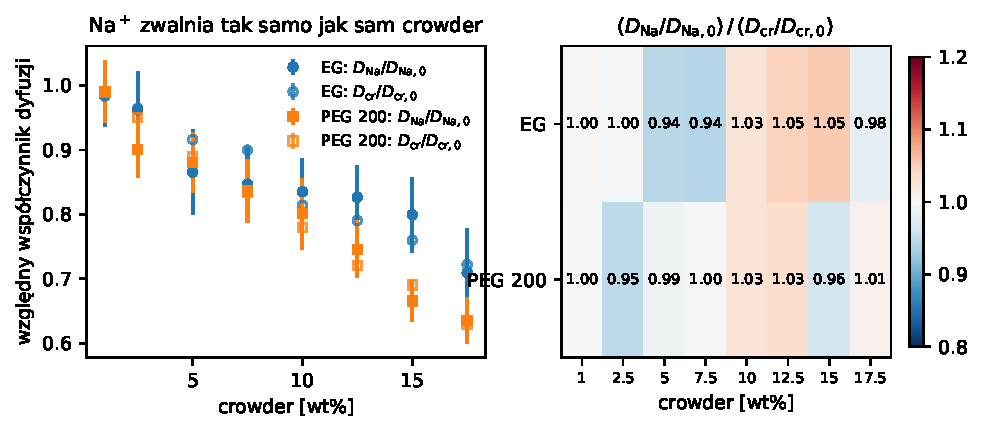
\includegraphics[width=0.92\linewidth]{t1_dosy_ratios.pdf}
\caption{EG i PEG 200: sód (pełne symbole) zwalnia tak samo jak sam crowder (puste). Mapa po prawej: stosunek obu spowolnień $\approx1$, czyli brak wiązania. Źródło: \texttt{knowles\_reframe/analysis.py}.}
\label{fig:dosy}
\end{figure}

\section{Nasze podejście (manuskrypt) i czego w nim brakuje}
\textbf{Co robimy.} Trzy kroki:
\begin{align}
c_\text{Na,eff} &= \frac{c_0}{1+\beta n\, c_\text{PEG}} &&\text{(„wolny” sód z NMR)}\\
\Delta\Delta G_\text{el} &= \Delta G_\text{hyb}(c_\text{Na,eff})-\Delta G_\text{hyb}(c_0) &&\text{(odczyt z krzywej solnej buforu)}\\
\Delta G_\text{rest} &= \Delta\Delta G_\text{obs}-\Delta\Delta G_\text{el} &&\text{(reszta przypisana deplecji)}
\end{align}

\textbf{Czego brakuje (od najważniejszego):}
\begin{enumerate}[leftmargin=*]
\item \textbf{DNA „czuje” sól jako całość, nie sam sód.} Hybrydyzacja nie zmienia ładunku DNA, więc ze ścisłej termodynamiki $d\ln K=S_K\,d\ln a_\pm$, gdzie $a_\pm=\sqrt{a_+a_-}$ (średnia aktywność kationu i anionu). Jeśli PEG wiąże tylko kation, właściwe stężenie do odczytu z krzywej to
$$c_\text{eq}=\frac{c_0}{\sqrt{1+\beta n\,c_\text{PEG}}},$$
a nie $c_0/(1+\beta n\,c_\text{PEG})$. W skali logarytmicznej nasz wzór daje więc \textbf{2 razy za dużo}.
\item \textbf{„Rozcieńczenie” buforu jest artefaktem.} W kodzie stężenie sodu spada z 35 do 22.5 mM przy 40 wt\% PEG. Próbki robimy jednak przez naważenie PEG i dodanie buforu, więc sól na kilogram wody się nie zmienia. To dodaje sztucznie około +3 kJ/mol.
\item \textbf{Anion jest pominięty, a literatura mówi, że jest kluczowy.} Pomiary VPO (ciśnienie pary) pokazują, że PEG \emph{wypycha} sól, głównie anion: dla grupy EO wkład Na$^+$ wynosi $+4.7$, Cl$^-$ $+37.6$, a HPO$_4^{2-}$ aż $+234$~cal\,mol$^{-1}$molal$^{-1}$ \cit{b:kn15}. Dodatnia wartość oznacza wypychanie, czyli \emph{wzrost} aktywności soli, który stabilizuje DNA. To kierunek odwrotny do naszego założenia.
\item \textbf{Zły kształt.} Wiązanie daje człon $\ln(1+\beta n c)$, który rośnie najszybciej na początku i potem słabnie (krzywa wklęsła). Obserwowana destabilizacja długich PEG przyspiesza ze stężeniem (wypukła). Sam sód nie może więc wytworzyć minimum i odwrócenia.
\item \textbf{Wielkość.} Udział członu solnego w odwróceniu stabilizacji długich PEG wynosi 69\% w obecnym kodzie, 20\% po poprawkach 1--2 i około 10--14\% przy mniejszych $\kappa$. Przy wypychaniu soli jak dla PEG--KCl jest to $-36\%$, czyli działa w przeciwną stronę (rys.~\ref{fig:var}).
\item \textbf{Brak testu.} Nigdzie nie sprawdzamy, czy efekt PEG zależy od stężenia soli tak, jak przewiduje mechanizm sodowy. Argument z pracy Bielec 2022 („dodanie soli przywraca $K$”) jest kołowy: te same dane służą do wyznaczenia $\kappa$ i do jego „potwierdzenia”, a dosypanie soli kompensuje \emph{każdą} destabilizację, niezależnie od jej przyczyny.
\end{enumerate}

\begin{figure}[h]
\centering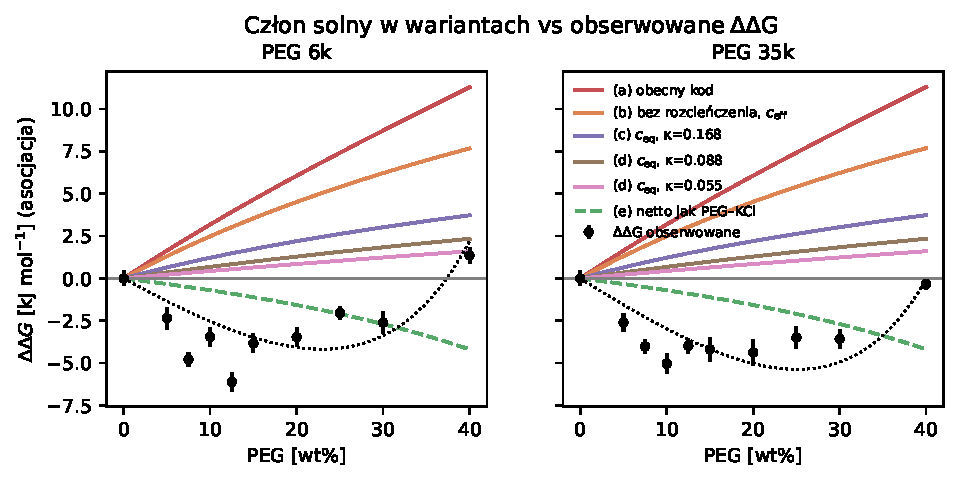
\includegraphics[width=0.92\linewidth]{t2_variants.pdf}
\caption{Człon solny w wariantach (a)--(e) dla PEG 6k i 35k na tle danych (punkty). Czerwony to obecny kod; fioletowy wersja poprawiona; zielony przerywany wypychanie soli jak u Knowlesa. Źródło: \texttt{knowles\_reframe/analysis.py}.}
\label{fig:var}
\end{figure}

\section{Podejście Knowlesa: krótko i matematycznie}
Knowles i in. \cit{b:kn11} mierzą topnienie 12-meru w EG i PEG 200--20\,000 i rozkładają efekt kosolutu na dwa człony. Wielkość podstawowa to \emph{m-wartość}, czyli nachylenie energii swobodnej względem molalności kosolutu $m_3$:
$$m\equiv\frac{\partial\Delta G^\circ_\text{obs}}{\partial m_3}=\Delta\mu_{23}=\Delta\mu^\text{pi}_{23}+\Delta\mu^\text{ev}_{23}.$$
\textbf{Oddziaływania preferencyjne} (pi) to słabe, korzystne kontakty grup glikolu z powierzchnią zasad, która odsłania się przy topnieniu. Liczy się je z pola powierzchni:
$$\frac{\Delta\mu^\text{pi}_{23}}{N}=\chi(N)\,\alpha_I\,\text{ASA}_I\,\Delta\text{ASA}_\text{DNA},$$
gdzie $N$ to liczba jednostek EO, $\alpha_I=-2.21\cdot10^{-6}$~kcal\,molal$^{-1}$Å$^{-4}$ (siła oddziaływania na Å$^2$), ASA$_I=82.5$~Å$^2$ (powierzchnia jednostki EO), $\Delta$ASA $\approx2006$~Å$^2$ (powierzchnia odsłaniana przy topnieniu), a $\chi$ to ułamek jednostek EO dostępnych dla DNA: 1 dla krótkich glikoli, $\chi_\infty=0.45$ dla długich łańcuchów (w reanalizie tej samej grupy 0.6 \cit{b:shkel}).

\textbf{Objętość wyłączona} (ev, deplecja) wg Hermansa:
$$\Delta\mu^\text{ev}_{23}=RT\rho_1\,\Delta V_{23},\qquad V_{23}=N\,l_k^2\,(10^{-27}N_A)\,k,$$
czyli dla długich łańcuchów wielkość stała \emph{na monomer}, niezależna od $M$ ($l_k=11.9$~Å, dla dupleksu $+0.309$~kcal/molal monomeru).

\textbf{Sól.} Poprawka na aktywność soli wynika z linkage'u:
$$\Big(\frac{\partial\ln K}{\partial m_3}\Big)_{a_\pm}=\Big(\frac{\partial\ln K}{\partial m_3}\Big)_{m_4}-\frac{S_K\,\mu_{34}}{2RT(1+\varepsilon)},$$
gdzie $\mu_{34}$ mierzą VPO. Dla PEG--KCl $\mu_{34}=+0.035$~kcal/molal monomeru, czyli wypychanie soli.

\textbf{Odwrócenie stabilizacji.} Powyżej około 6 molal monomeru (około 21 wt\%) łańcuchy się przeplatają, DNA „widzi” krótkie odcinki PEG, $\chi\to1$, a destabilizacja na monomer wraca do wartości dla PEG 200.

\textbf{Liczby Knowlesa a nasze dane, bez żadnego dopasowania} (rys.~\ref{fig:kn}): EG 40\% $+15.3$ vs zmierzone $+14.7$~kJ/mol; PEG 200 40\% $+13.3$ vs $+13.6$; PEG 35k przy 20\% $-3.7\ldots-5.9$ vs $-4.4$. Różnica jest tylko na początku: nasza stabilizacja narasta 2--3 razy szybciej do około 5 wt\%.

\textbf{Słabe punkty Knowlesa:} oddziaływań glikol--zasada nikt nie zaobserwował bezpośrednio (wynikają z termodynamiki); objętość wyłączona pochodzi z teorii dla łańcuchów idealnych; poprawka solna oparta jest na VPO tylko dla PEG 1000/2000 z KCl.

\begin{figure}[h]
\centering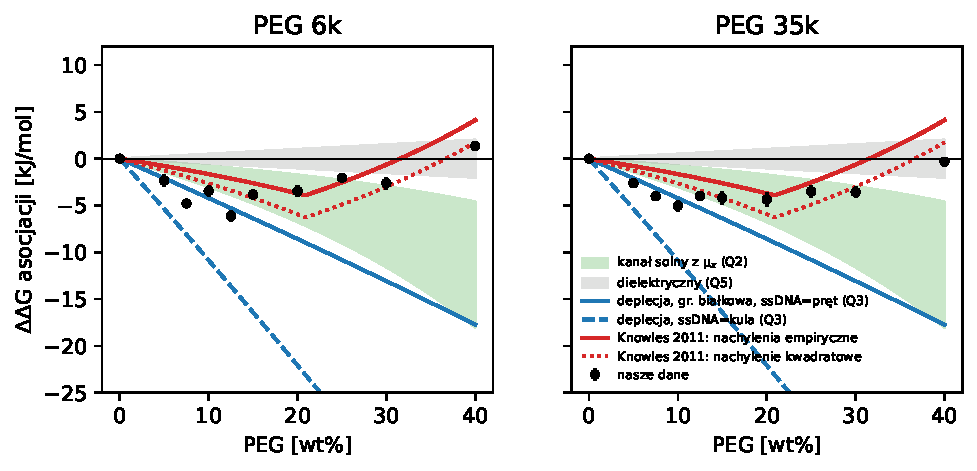
\includegraphics[width=0.92\linewidth]{lit_budget.pdf}
\caption{Nasze dane (punkty) vs człony z literatury bez dopasowania: nachylenia Knowlesa (czerwone), deplecja w teorii polimerów (niebieskie), kanał solny z VPO (zielony), stała dielektryczna (szary). Źródło: \texttt{literature\_check/lit\_budget.py}.}
\label{fig:kn}
\end{figure}

\clearpage
\section{Jak to rozstrzygnąć: przesunięcie poziome czy pionowe}
\subsection{Idea}
Narysujmy $\ln K$ w funkcji $\ln c_\text{Na}$ (krzywa solna). W buforze ma ona maksimum przy około 150 mM. Kosolut może ją zmienić na trzy sposoby:
\begin{itemize}[leftmargin=*]
\item \textbf{A, przesunięcie poziome} (zmiana aktywności soli): $\ln K(c,x)=F(\ln c-\varphi)$. Wiązanie sodu przesuwa krzywą w prawo, wypychanie soli w lewo.
\item \textbf{B, przesunięcie pionowe} (efekt niezależny od soli, np. oddziaływania z zasadami, deplecja): $\ln K=F(\ln c)+H$.
\item \textbf{C, zmiana nachylenia} (DNA staje się mniej czułe na sól, np. przez niższą stałą dielektryczną): krzywa „spłaszcza się”.
\end{itemize}
Na prostym odcinku krzywej A i B wyglądają identycznie. Różnią się tam, gdzie krzywa się wygina, zwłaszcza w maksimum: \textbf{tylko A przesuwa położenie maksimum} (rys.~\ref{fig:abc}).

\begin{figure}[h]
\centering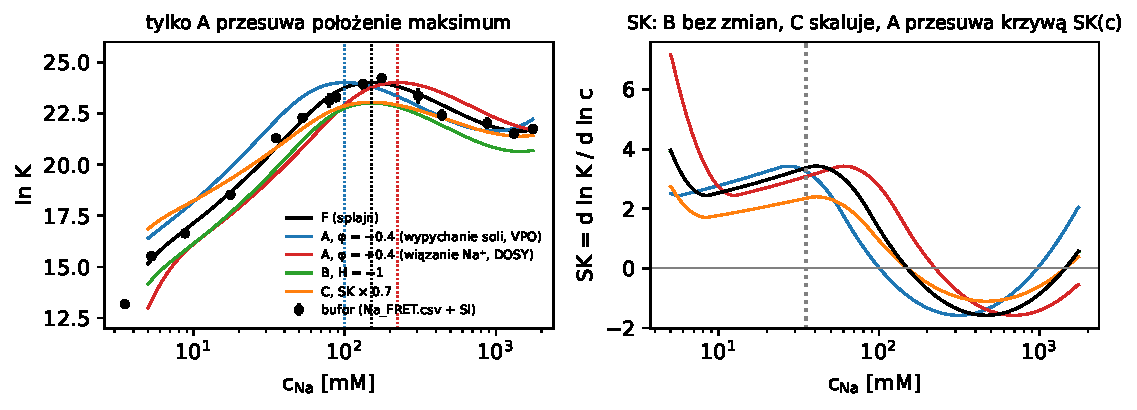
\includegraphics[width=0.9\linewidth]{predictions_ABC.pdf}
\caption{Przewidywania na naszej krzywej buforu: A przesuwa maksimum (100 lub 224 mM zamiast 151 mM), B obniża krzywą, C zmniejsza nachylenie (przy 35 mM z 3.38 do 2.36). Skrypt \texttt{predictions\_ABC.py}.}
\label{fig:abc}
\end{figure}

\subsection{Co już zrobiono w literaturze}
\begin{itemize}[leftmargin=*]
\item \textbf{Nikt nie przeszedł z solą przez maksimum w obecności kosolutu.} Najbliżej są Nakano 2004 i Ghosh 2020, ale mają tylko dwa stężenia soli (0.12 i 1 M) \cit{b:nak04,b:gh20}.
\item \textbf{Rozdział „przez sól” i „bezpośrednio” już robiono}, ale człon solny mierzono przez VPO, a nie samym DNA (szkoła Recorda \cit{b:hong05}; Lambert, Leipply i Draper \cit{b:llld10,b:ld12}). Lambert i in. pokazali, że kosolut może zmienić nachylenie bez zmiany aktywności soli, czyli przez mechanizm C.
\item \textbf{Powtarzalny wzór dla PEG:} nachylenie maleje (Markarian 2010: 2.96 $\to$ 1.35; Nakano 2014: 1.54 $\to$ 1.14), a stabilizacja przez długi PEG słabnie z solą aż do przecięcia krzywych \cit{b:mark,b:nak14} (rys.~\ref{fig:lit}). To B + C. Nigdzie nie widać śladu wiązania sodu.
\item \textbf{Mg$^{2+}$ i RNA:} „PEG obniża potrzebne Mg$^{2+}$”, czyli przesunięcie poziome. Autorzy sprawdzili przez VPO, że to nie zmiana aktywności jonów, i przypisali je objętości wyłączonej \cit{b:kil10,b:desai}.
\end{itemize}

\begin{figure}[h]
\centering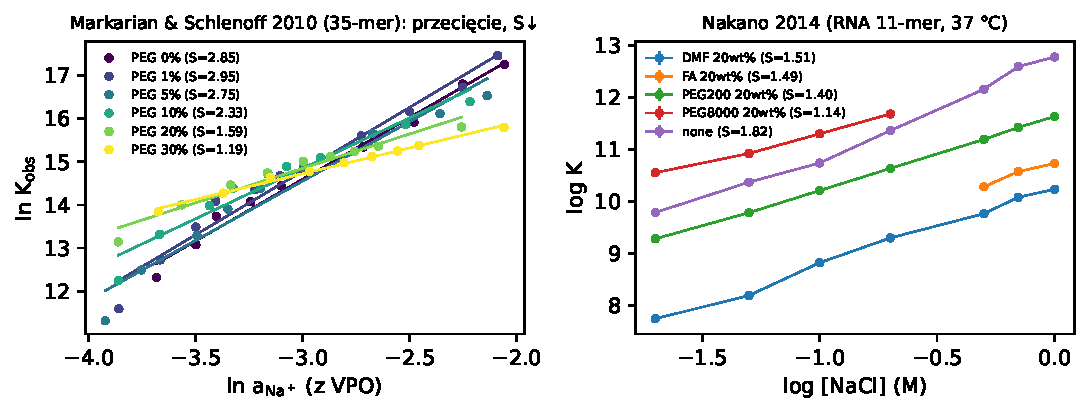
\includegraphics[width=0.92\linewidth]{lit_replot.pdf}
\caption{Dane z literatury zdigitalizowane w tym przeglądzie. Lewo: długi PEG zmniejsza nachylenie i krzywe się przecinają. Prawo: PEG 8000 i PEG 200 obniżają nachylenie. Skrypt \texttt{lit\_replot.py}.}
\label{fig:lit}
\end{figure}

\subsection{Bielec 2022 w tej ramie}
Zdigitalizowaliśmy Fig.~S3 (K w funkcji Na$^+$ w 40 wt\% crowderów). Wnioski:
\begin{itemize}[leftmargin=*]
\item Zakres 10--125 mM leży w całości poniżej maksimum, a krzywa buforu w pracy to dopasowanie potęgowe (stałe nachylenie 2.51). \textbf{Na takiej referencji A i B są nie do odróżnienia}, a cała metoda wyznaczania $\kappa$ zakłada A.
\item Nachylenia w crowderach są jednak inne niż w buforze: EG $1.32\pm0.06$, dekstrany i Ficoll 1.8--2.2, PEG 400 około 2.1. To sygnatura C, której model „wiązania” nie przewiduje.
\item Dla EG „ułamek związanego sodu” wyliczony metodą pracy rośnie z 0.62 do 0.88 wraz ze stężeniem soli, a powinien być stały. Założenie pracy jest więc niespójne z jej własnymi danymi.
\end{itemize}

\begin{figure}[h]
\centering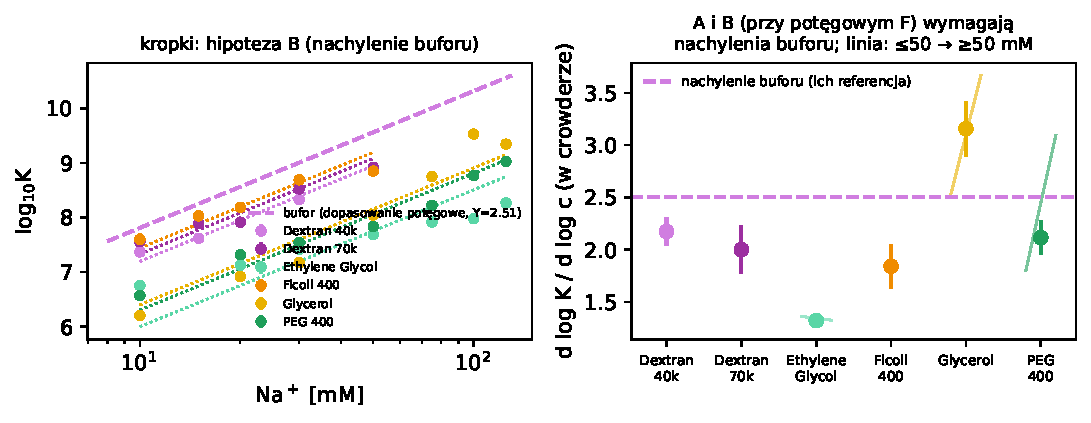
\includegraphics[width=0.92\linewidth]{ab_bielec_s3.pdf}
\caption{Bielec 2022, Fig.~S3 zdigitalizowana. Lewo: dane i hipoteza B (kropki). Prawo: nachylenia w crowderach vs nachylenie buforu (linia przerywana). Skrypt \texttt{ab\_bielec\_s3.py}.}
\end{figure}

\subsection{Plan naszego eksperymentu}
\begin{enumerate}[leftmargin=*]
\item \textbf{Krzywa solna przez maksimum:} bufor, EG 20 i 40\%, PEG 400 40\%, PEG 35k 10\%; Na$^+$: 10, 20, 35, 50, 75, 100, 150, 200, 300, 450, 600 mM.
\item \textbf{Co mierzymy:} położenie maksimum (A je przesuwa, B i C nie), nachylenie przy 35 mM (C je obniża), przesunięcie w pionie (B). Dopasowanie globalne trzech parametrów $\varphi$, $H$, $\lambda$ dla każdego crowdera.
\item \textbf{Niezależna kontrola:} VPO soli z PEG/EG w naszym buforze, które daje $\varphi$ bez DNA.
\item \textbf{Pułapki:} w maksimum $K\approx3\cdot10^{10}$, czyli na granicy oznaczalności przy 10 nM donora (użyć 1 nM donora albo warunków o niższym $K$); możliwy rozdział faz PEG + sól; para FRET może sama reagować na sól i crowder (kontrola z jednym znacznikiem).
\end{enumerate}

\ramka{\textbf{Co z tego wynika dla manuskryptu.} Mechanizm „PEG wiąże sód” nie ma dziś niezależnego potwierdzenia i ma przeciwko sobie pomiary termodynamiczne (VPO). Bezpieczniej opisać dane w ramie Knowlesa (oddziaływania z zasadami + objętość wyłączona), a wiązanie sodu z NMR przedstawić jako obserwację o progowej zależności od długości łańcucha, której wpływ na $K$ trzeba dopiero zmierzyć proponowanym eksperymentem.}

\section*{Bibliografia}
\small
\begin{enumerate}[label={[\arabic*]},ref={\arabic*},leftmargin=*,itemsep=0pt]
\item\label{b:kn11} Knowles D.B., LaCroix A.S., Deines N.F., Shkel I., Record M.T. Jr. Separation of preferential interaction and excluded volume effects on DNA duplex and hairpin stability. \emph{PNAS} 108, 12699 (2011). DOI 10.1073/pnas.1103382108.
\item\label{b:kn15} Knowles D.B., Shkel I.A., Phan N.M., et al., Record M.T. Jr. Chemical Interactions of Polyethylene Glycols (PEGs) and Glycerol with Protein Functional Groups: Applications to Effects of PEG and Glycerol on Protein Processes. \emph{Biochemistry} 54, 3528 (2015). DOI 10.1021/acs.biochem.5b00246.
\item\label{b:shkel} Shkel I.A., Knowles D.B., Record M.T. Jr. Separating chemical and excluded volume interactions of polyethylene glycols with native proteins: Comparison with PEG effects on DNA helix formation. \emph{Biopolymers} 103, 517 (2015). DOI 10.1002/bip.22662.
\item\label{b:nak04} Nakano S., Karimata H., Ohmichi T., Kawakami J., Sugimoto N. The Effect of Molecular Crowding with Nucleotide Length and Cosolute Structure on DNA Duplex Stability. \emph{J. Am. Chem. Soc.} 126, 14330 (2004). DOI 10.1021/ja0463029.
\item\label{b:gh20} Ghosh S., Takahashi S., Ohyama T., Endoh T., Tateishi-Karimata H., Sugimoto N. Nearest-neighbor parameters for predicting DNA duplex stability in diverse molecular crowding conditions. \emph{PNAS} 117, 14194 (2020). DOI 10.1073/pnas.1920886117.
\item\label{b:nak14} Nakano S., Kitagawa Y., Miyoshi D., Sugimoto N. Hammerhead ribozyme activity and oligonucleotide duplex stability in mixed solutions of water and organic compounds. \emph{FEBS Open Bio} 4, 643 (2014). DOI 10.1016/j.fob.2014.06.009.
\item\label{b:mark} Markarian M.Z., Schlenoff J.B. Effect of Molecular Crowding and Ionic Strength on the Isothermal Hybridization of Oligonucleotides. \emph{J. Phys. Chem. B} 114, 10620 (2010). DOI 10.1021/jp103213w.
\item\label{b:llld10} Lambert D., Leipply D., Draper D.E. The Osmolyte TMAO Stabilizes Native RNA Tertiary Structures in the Absence of Mg$^{2+}$: Evidence for a Large Barrier to Folding from Phosphate Dehydration. \emph{J. Mol. Biol.} 404, 138 (2010). DOI 10.1016/j.jmb.2010.09.043.
\item\label{b:ld12} Lambert D., Draper D.E. Denaturation of RNA Secondary and Tertiary Structure by Urea: Simple Unfolded State Models and Free Energy Parameters Account for Measured m-Values. \emph{Biochemistry} 51, 9014 (2012). DOI 10.1021/bi301103j.
\item\label{b:hong05} Hong J., Capp M.W., Saecker R.M., Record M.T. Jr. Use of Urea and Glycine Betaine To Quantify Coupled Folding and Probe the Burial of DNA Phosphates in Lac Repressor$-$Lac Operator Binding. \emph{Biochemistry} 44, 16896 (2005). DOI 10.1021/bi0515218.
\item\label{b:kil10} Kilburn D., Roh J.H., Guo L., Briber R.M., Woodson S.A. Molecular Crowding Stabilizes Folded RNA Structure by the Excluded Volume Effect. \emph{J. Am. Chem. Soc.} 132, 8690 (2010). DOI 10.1021/ja101500g.
\item\label{b:desai} Desai R., Kilburn D., Lee H.-T., Woodson S.A. Increased Ribozyme Activity in Crowded Solutions. \emph{J. Biol. Chem.} 289, 2972 (2014). DOI 10.1074/jbc.M113.527861.
\item\label{b:bielec22} Bielec K., Kowalski A., Bubak G., Witkowska Nery E., Hołyst R. Ion Complexation Explains Orders of Magnitude Changes in the Equilibrium Constant of Biochemical Reactions in Buffers Crowded by Nonionic Compounds. \emph{J. Phys. Chem. Lett.} 13, 112 (2022). DOI 10.1021/acs.jpclett.1c03596.
\end{enumerate}
Wszystkie DOI sprawdzone w Crossref; pełne listy z oznaczeniem dostępu w \texttt{salt\_shift/\{na,mg\}\_notes.md} i \texttt{literature\_check/notes/}.
\end{document}
